\documentclass[12 pt]{report}
\usepackage[english]{babel}
\usepackage{fancyhdr}
\usepackage{amsmath}
\usepackage{bm}
\usepackage{tabularx}
\usepackage{hyperref}
\usepackage{graphicx}
\usepackage{amsfonts}
\usepackage{color}   %May be necessary if you want to color links
\usepackage{hyperref}
\hypersetup{
    colorlinks=true, %set true if you want colored links
    linktoc=all,     %set to all if you want both sections and subsections linked
    linkcolor=blue,  %choose some color if you want links to stand out
}
\graphicspath{ {images/} }


\pagestyle{fancy}
\fancyhf{}
\rhead{Machine Learning}
\lhead{Summer of Science}
\cfoot{\thepage}


\title{
    {\textbf{Midsem Report: Machine Learning}}\\
    {\large Summer of Science 2022}\\
}
\author{Ashwin Abraham}
\date{19th June, 2022}

\begin{document}
    \maketitle
    \tableofcontents

    \chapter{Linear and Logistic Regression}
    Regression is the statistical process to find the relationship between a dependent variable and an independent variable that minimizes some 
    cost function, given a set of datapoints.


    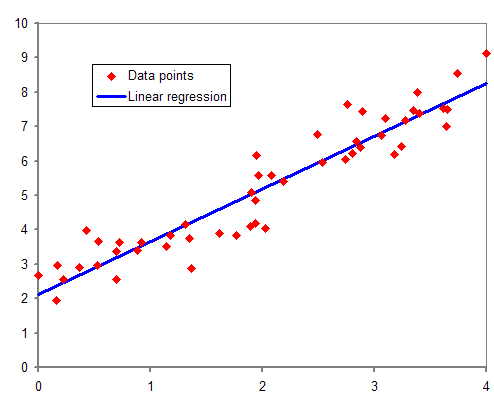
\includegraphics[scale = 0.7]{Normdist_regression}


    The above graph shows an example of Linear Regression with one dependent and one independent variable, where a set of datapoints is given, and we try to find the line that best represents the
    relationship between the dependent variable and the independent variable.

    The notion of what we mean by "best representation" is formalized by the cost function. This is a function of the dataset given to us and the 
    approximate relationship we use to model the relationship between the dependent and independent variables. The best representation of this 
    relation is the one that has the least cost (minimizes the value of the cost function).

    \section{Linear Regression}

    In linear regression, we impose the constraint that approximate relationship between the dependent and independent variables should be a linear 
    function. The cost function usually chosen for regression problems is the sum of squares function (leading the method itself to be called the 
    method of least squares). 

    If there are $N$ datapoints of the form $(x_{i}, y_{i})$ and the relation function is $f$, then the cost of $f$ is then  defined as:
    \begin{equation}
        C(f) = \sum_{i = 1}^{n} ||y_{i} - f(x_{i})||^{2}
    \end{equation}
    Here, if there are more than $1$ dependent/independent variable, $x$ and $y$ become vectors.

    Assuming $f$ is linear and there are only $1$ dependent and $1$ independent variable, we get $f(x) = Ax + B$. Now we must find constants $A$ and $B$ such that $C(f) = C(A, B)$ is minimized. Now,
    \begin{equation}
        C(A, B) = \sum_{i = 1}^{n} (y_{i} - Ax_{i} - B)^{2}
    \end{equation}
    Imposing the conditions that $\frac{\partial C}{\partial A} = \frac{\partial C}{\partial B} = 0$, we get
    \begin{equation}
        \sum_{i = 1}^{n} (Ax_{i} + B - y_{i})x_{i} = 0
    \end{equation}
    and
    \begin{equation}
        \sum_{i = 1}^{n} (Ax_{i} + B - y_{i}) = 0
    \end{equation}
    Simplifying, we get a system of Linear equations in $A$ and $B$:
    \begin{equation}
        A(\sum_{i = 1}^{n} x_{i}^{2}) + B(\sum_{i = 1}^{n} x_{i}) = \sum_{i = 1}^{n} x_{i}y_{i}
    \end{equation}
    \begin{equation}
        A(\sum_{i = 1}^{n} x_{i}) + Bn = \sum_{i = 1}^{n} y_{i}
    \end{equation}

    Note, that since in the RMS-AM inequality ($n(\sum_{i = 1}^{n} x_{i}^{2}) \geq (\sum_{i = 1}^{n} x_{i})^{2}$), equality occurs only when all 
    $x_{i}$ are equal (which can never happen with a proper data set), this equation will always have a unique solution, given by:
    \begin{equation}
        A = \frac{n(\sum x_{i}y_{i}) - (\sum x_{i})(\sum y_{i})}{n(\sum x_{i}^{2}) - (\sum x_{i})^{2}}
    \end{equation}
    \begin{equation}
        B = \frac{(\sum y_{i})(\sum x_{i}^{2}) - (\sum x_{i}y_{i})(\sum x_{i})}{n(\sum x_{i}^{2}) - (\sum x_{i})^{2}}
    \end{equation}

    \section{Logistic Regression}
    In a logistic regression on the other hand, the dependent variable is constrained to be only either $0$ or $1$.
    In this case, the best approximation to the relation between the dependent and independent variables will also be the
    Probability Function of the dependent variable (this is a function of the independent variables that gives the probability 
    that the dependent variable will be $1$ for a particular choice of independent variables).



    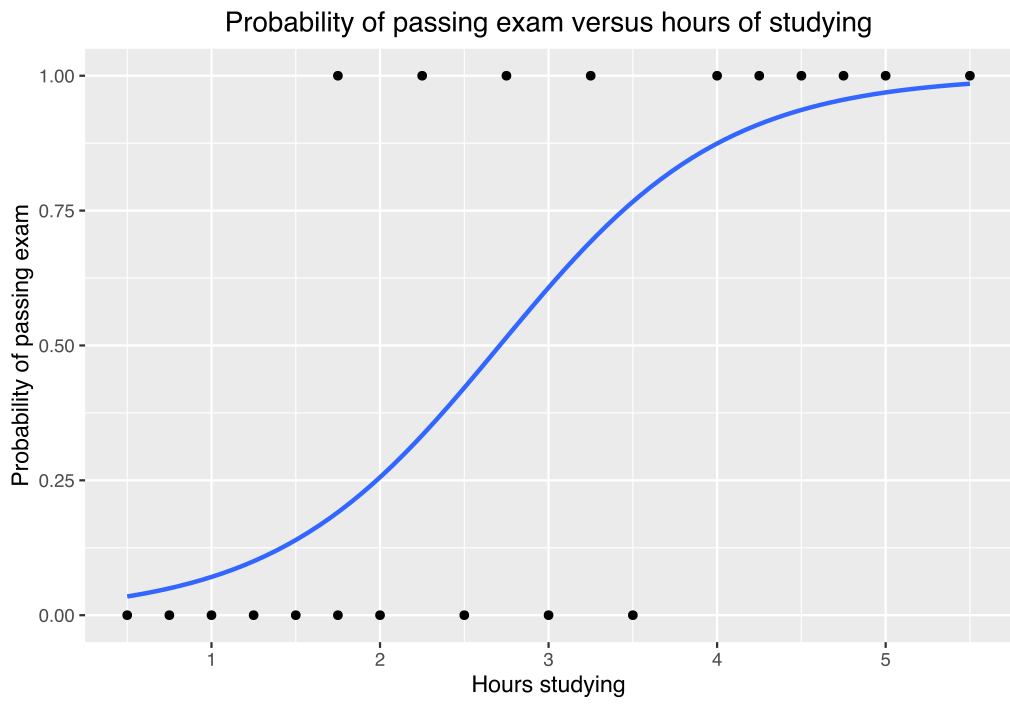
\includegraphics[scale = 0.55]{logistic.png}

    The above graph shows an example of a Probability function obtained by Logistic Regression.
    
    The cost function for Logistic Regression is given by:
    \begin{equation}
        C(p) = -\sum_{i = 1}^{n} [y_{i}\ln(p(x_{i})) + (1-y_{i})\ln(1 - p(x_{i}))]
    \end{equation}

    and we model the relation between the dependent and independent variables by a logistic function, given by:
    \begin{equation}
        p(x) = \frac{1}{1 + \exp(-(Ax + B))}
    \end{equation}

    Now, expressing $C$ in terms of $A$ and $B$ and then imposing the condition that $\frac{\partial C}{\partial A} = \frac{\partial C}{\partial B} = 0$, 
    we get the values of $A$ and $B$. Note that the equations involved may not always have exact solutions and may have to be solved numerically.

    \section{Use of Regression in Machine Learning}
    A system implementing Machine Learning techniques must be trained with a large amount of data and it must use the data it has been trained with 
    in order to find ways of handling data that it has not come across before. This can be done effectively using regression techniques. The Machine 
    can use regression analysis on the training data to get a relation between the data and the desired outcome. If the outcome is a binary decision, 
    Logistic regression may be used, and if it is a continuous outcome, Linear regression may be used. The relation obtained is applied on the new data 
    to get the outcome required.

    \chapter{Support Vector Machines}
    In Machine Learning, we often need to classify data into multiple groups. If the data can be represented as an $n$-dimensional vector, then 
    the dataset becomes a set of points in $\mathbb{R}^{n}$. The easiest way to classify data into different groups is to find a $n$-dimensional 
    hyperplane dividing the $\mathbb{R}^{n}$ into two parts, one containing one set of points and another containing the remaining points.

    To find the hyperplane, we use a set of points that have already been preclassified into two groups and try to find a hyperplane that separates the two 
    groups into two halves of $\mathbb{R}^{n}$. 
    If such a hyperplane exists, the dataset (along with the grouping) is said to be Linearly Separable.
    If a hyperplane exists, then (assuming that the number of points is finite), then an infinite number of such hyperplanes exist.
    We therefore, choose the hyperplane with the maximum margin, where the margin is defined as the max(minimum distance to a point on one side, minimum distance to a point on the other), 
    as illustrated in the following figure:


    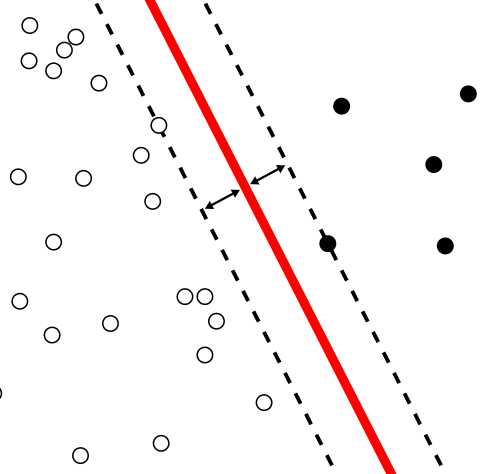
\includegraphics[scale = 1.2]{margin.png}

    For the training set of points $\bm{x_{1}}$, $\bm{x_{2}}$ $\cdots$, $\bm{x_{n}}$, where $\bm{x_{i}} \in \mathbb{R}^{m}$, consider the function 
    $y$ defined as:
    \begin{equation}
        y(\bm{x}) = \begin{cases}
            1 &, \bm{x} \in \text{Group 1} \\
            -1 &, \bm{x} \in \text{Group 2}
        \end{cases}
    \end{equation}

    We can write the equation of the separating plane with the maximum margin as $\bm{w}^{T}\bm{x} = b$ where $\bm{w}$ is an arbitrary non-null vector in 
    $\mathbb{R}^{m}$ and $b$ is an arbitrary real number.

    \section{Linearly Separable Data}
    If the dataset is linearly separable, then there exist two parallel margin planes passing through the closest points to the separating plane.
    The seperating plane will also be parallel to this plane and will be exactly between the two planes. Therefore, we can have appropriate $\bm{a}$ 
    and $b$ such that the two margin planes are given by $\bm{a}^{T}\bm{x} - b = 1$ for the separating plane passing through the closest point in 
    Group $1$ and $\bm{a}^{T}\bm{x} - b = -1$ for the separating plane passing through the closest point in Group $2$.


    The distance between the margins here is given by $d = \frac{2}{||\bm{a}||}$, which is the quantity to be maximized (i.e. $||\bm{a}||$ must be minimized).
    Imposing the condition that all the points in group $1$ lie on the opposite side of $\bm{a}^{T}\bm{x} - b = 1$ as $\bm{a}^{T}\bm{x} - b$ and similiarly for 
    the points in group $2$ and $\bm{a}^{T}\bm{x} - b = -1$.

    This condition may be expressed as:
    \begin{equation}
        y(\bm{x_{i}})(\bm{a}^{T}\bm{x_{i}} - b) \geq 1, \forall i \in \{1 \cdots n\}
    \end{equation}

    If we know the two closest points to the separating plane (from opposite sides) (say $\bm{x_{a}}$ and $\bm{x_{b}}$), we can reduce these constrained minimization problem to 
    minimizing $||\bm{a}||$ based on the constraints:
    \begin{equation}
        y(\bm{x})(\bm{a}^{T}\bm{x} - b) = 1, \bm{x} \in \{\bm{x_{a}}, \bm{x_{b}}\}
    \end{equation}

    $\bm{x_{a}}$ and $\bm{x_{b}}$ are known as support vectors (hence the name Support Vector Machine). $\bm{a}$ and $b$ obtained are clearly dependent only 
    on the Support Vectors.

    \section{Non-Separable Data}
    For data that is not linearly separable, a separating plane doesn't exist that clearly divides space into regions containing only points of the same group.
    However, it is still possible for there to exist a plane that roughly divides space into regions containing points mostly of the same types. We can still 
    use this plane to make predictions about points not in our data.

    Instead of minimizing $||\bm{a}||$, we instead minimize the quantity:
    \begin{equation}
        k||\bm{a}||^{2} + \frac{1}{n}\sum_{i = 1}^{n}[H(\bm{a}^{T}\bm{x_{i}} - b, y(\bm{x_{i}}))]
    \end{equation}
    for parameters $k$ and then choose the most appropriate $k$.

    Here $H$ represents the hinge function, defined as:
    \begin{equation}
        H(p, q) = max(0, 1-pq)
    \end{equation}
    Clearly, if $y(\bm{x_{i}})(\bm{a}^{T}\bm{x_{i}} - b) \geq 1$ then $H = 0$, i.e., if the points are on the correct side of the plane, there is no increase in the quantity to be minimized.
    If they are on the wrong side, then there is an increase, which is \textbf{proportional} to the degree in which the points are in the wrong side.

    The following is a graph of the Hinge function for $q = \frac{1}{2}$:

    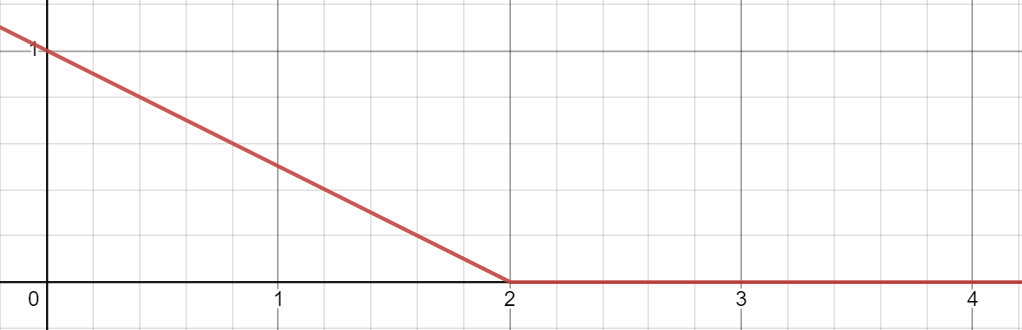
\includegraphics[scale = 0.8]{hinge.png}

    \chapter{Updated Plan of Action}
    \section*{\centering {Timeline}}
    \begin{center}
        \begin{tabularx}{0.8\textwidth}
            {
                |>{\centering\arraybackslash}X 
                |>{\centering\arraybackslash}X
                |>{\centering\arraybackslash}X
            }
            \hline
                \textbf{Dates} & \textbf{Topics to be covered} \\
            \hline
                16th June - 20th June & Principal Component Analysis, K-means clustering and Decision Trees (with Bagging and Boosting) \\
            \hline
                21st June - 25th June & Neural Networks and Convolutional Neural Networks \\
            \hline
                27th June - 1st July & (Endsems) \\
            \hline
                2nd July - 4th July & Recurrent Neural Networks \\
            \hline
                5th July - 7th July & Autoencoders \\
            \hline
                8th July - 11th July & Recommender Systems \\
            \hline
                12th July - 15th July & Final Report \\
            \hline
        \end{tabularx}
    \end{center}

    \section*{\centering {References}}
    \begin{enumerate}
        \item \href{https://www.coursera.org/learn/machine-learning#syllabus}{A basic ML course with minimal maths to get started with}
        \item \href{https://www.coursera.org/specializations/deep-learning#courses}{A five-course deep learning specialization by Coursera}
        \item \href{https://youtube.com/playlist?list=PLl8OlHZGYOQ7bkVbuRthEsaLr7bONzbXS}{This is an advanced course on Machine Learning by Cornell University with a good amount of focus on maths}
        \item \href{https://www.tensorflow.org/tutorials}{Tensorflow tutorial page has numerous implemented examples}
        \item \href{https://www.youtube.com/watch?v=_PwhiWxHK8o}{Follow this lecture series for learning Support Vector Machine (SVMs) and other topics which you find to be good in this series}
    \end{enumerate}
\end{document}